\chapter{Introduction}
The idea behind this project was to try to validate a startup idea by making use of simulation models. Specifically by leveraging an agent-based simulation.
In the report therefore we will go over what StiroApp is, how it works, the models that have been used as well as the technical implementation. Through the use of KPIs we will study the performance indicators of the model. After that there will be a chapter dedicated to experiments and finally the conclusions that can be drawn from it.

\section{StiroApp - The story behind}
StiroApp was born from the desire to bring to the market of applications, and more generally of services, a system that can connect two categories of people: Workers and Buyers. In more detail, the service seeks to make the process of ironing/washing one's clothing faster, more streamlined and more economical. I started by analyzing people's desire/problems by going to create user-stories necessary to make the product as user-centric as possible. As an example I reported one user story for a better understanding of the problem.
\subsection{User story - Max}
\begin{itemize}
\item \textbf{Context}: Max is a 27-year-old boy. He has been living alone for about a year. He moved to Milan for work reasons. He's a video game enthusiast.
\item \textbf{Problems:} 
	\begin{itemize}
		\item Because of his busy life, He does not have time to iron/wash his clothes
		\item It is a time-consuming, tedious and even difficult activity
	\end{itemize}
\end{itemize}
\section{Understanding the problem - More deeply}
After a series of dutiful analyses and interviews at the front to examine the problem as best as possible here is what can be extracted in a more abstract way representing the basic principles for which is Stirapp should be born.
\begin{itemize}
\item Only a few millennials make use of laundries
\item Daily laundry/ironing cannot be delegated to laundries
\item This type of daily activity (ironing/washing) is generally carried out by generation X (1965 - 1980) as opposed to generation Y (1980 - 1994) and Z (1995 - 2010)
\item Delivery/collection times of clothes are high
\end{itemize}
\section{Proposed solution}
The approach taken to solve these problems was therefore to offer an application for people in such a way as to connect the two categories into which we can classify users:
\begin{itemize}
\item Workers: Those who intend to use the application for the purpose of earning money by working for Buyers, thus ironing or washing their clothes.
\item Buyers: Those who intend to use the app as a service where they can get their laundry cleaned and ironed.
\end{itemize}
\subsection{Starting features}
The app can be divided into two major features:
\begin{itemize}
\item Create posts for your own clothes by specifying the type of service you want (example: washing, ironing, both) and your needs.
\item Wash, iron other users' clothes in such a way as to earn money.
\end{itemize}
\subsection{App Flow}
Below I show how the app should work. As an example during the agent-based simulation, some changes were made so as to focus more on the important parts of the app such as post creation or the worker system.
\begin{figure}[hbtp]
\caption{App flow Schema}
\centering
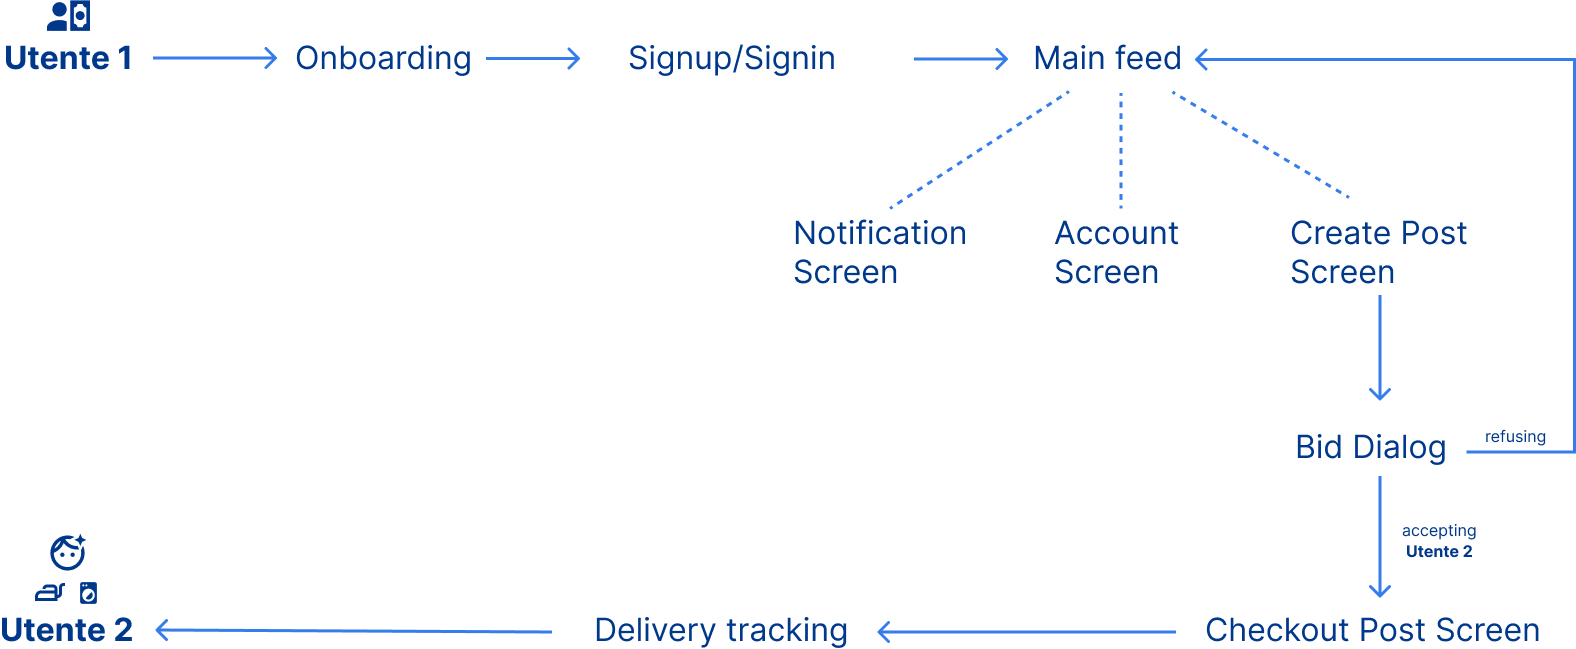
\includegraphics[scale=0.2]{../Images/AppFlow.png} 
\end{figure}
\begin{itemize}
\item \textbf{Utente 1 (Buyers)} enter in the app after the onboarding in which he can understand the main features of the app
\item \textbf{In-app onboarding} is the process of teaching users how to use an app to achieve their goals
\item \textbf{Signup-Signin}. The user must be logged or registered into the system before using the app 
\item The user will be redirect into the Main Screen of the app. Then with a bottom navigation bar he can choose in which page enter such us Notification screen, Account screen and the Create Post screen.
\item \textbf{Bid system} is a hypothetical part of the app in development
\item \textbf{Checkout post screen} is the confirm page after the accepted price
\item \textbf{Delivery tracking} is an important page for the user in order to check where is his order
\item \textbf{Utente 2} he is the Worker that is allowed to do the laundry or offer other type of services specified in the app during the create post screen
\end{itemize}
\subsection{UX and UI for StiroApp}
Before we get our hands on the code, it is important to study the user experience (UX) and user interface (UI) to finalize the creation of a user-friendly application.
So here I report some images of the work done:
\begin{figure}[hbtp]
\caption{Representation of the main features of the application through UX}
\centering
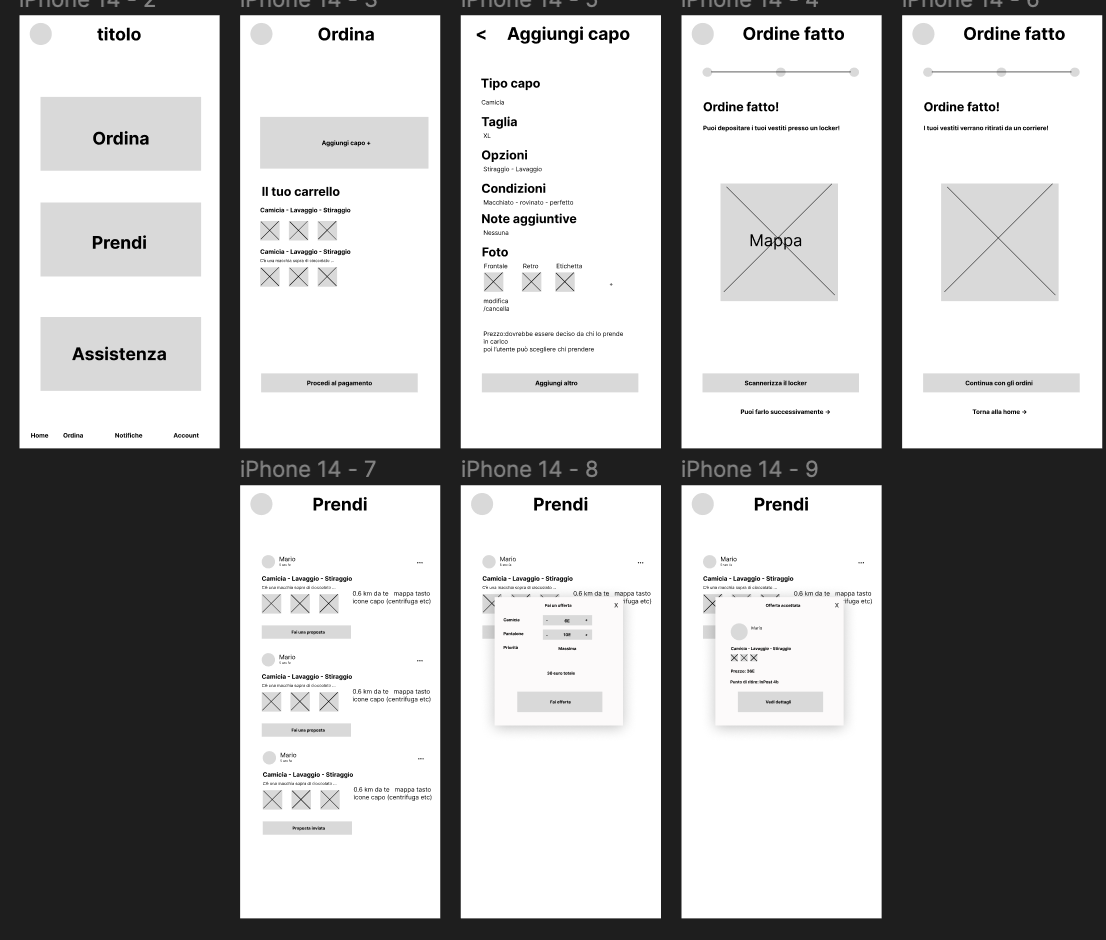
\includegraphics[scale=0.5]{../Images/ux.png}
\end{figure}
\begin{figure}[hbtp]
\caption{An example of Card UI for the post creation}
\centering
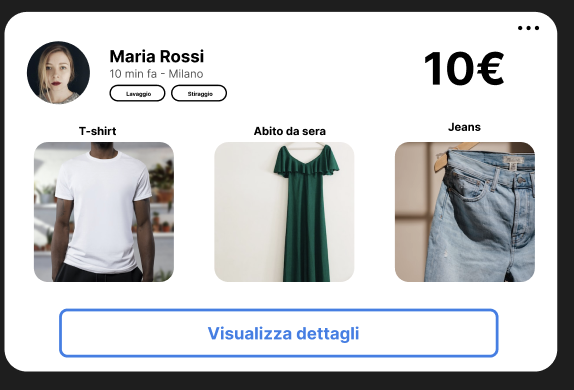
\includegraphics[scale=0.5]{../Images/cardui.png}
\end{figure}
\subsection{Mockup}
To give a real representation of StirApp to the reader I created a mockup. According to Decode Agency \cite{decodeagency}, an app mockup is a detailed representation of your app design. It contains all the final UI elements such as typography, copy, colors, and visuals like icons and photos. Sample content will also be used, but dummy text is also acceptable.
\begin{figure}[hbtp]
\caption{Main Feed Mockup}
\centering
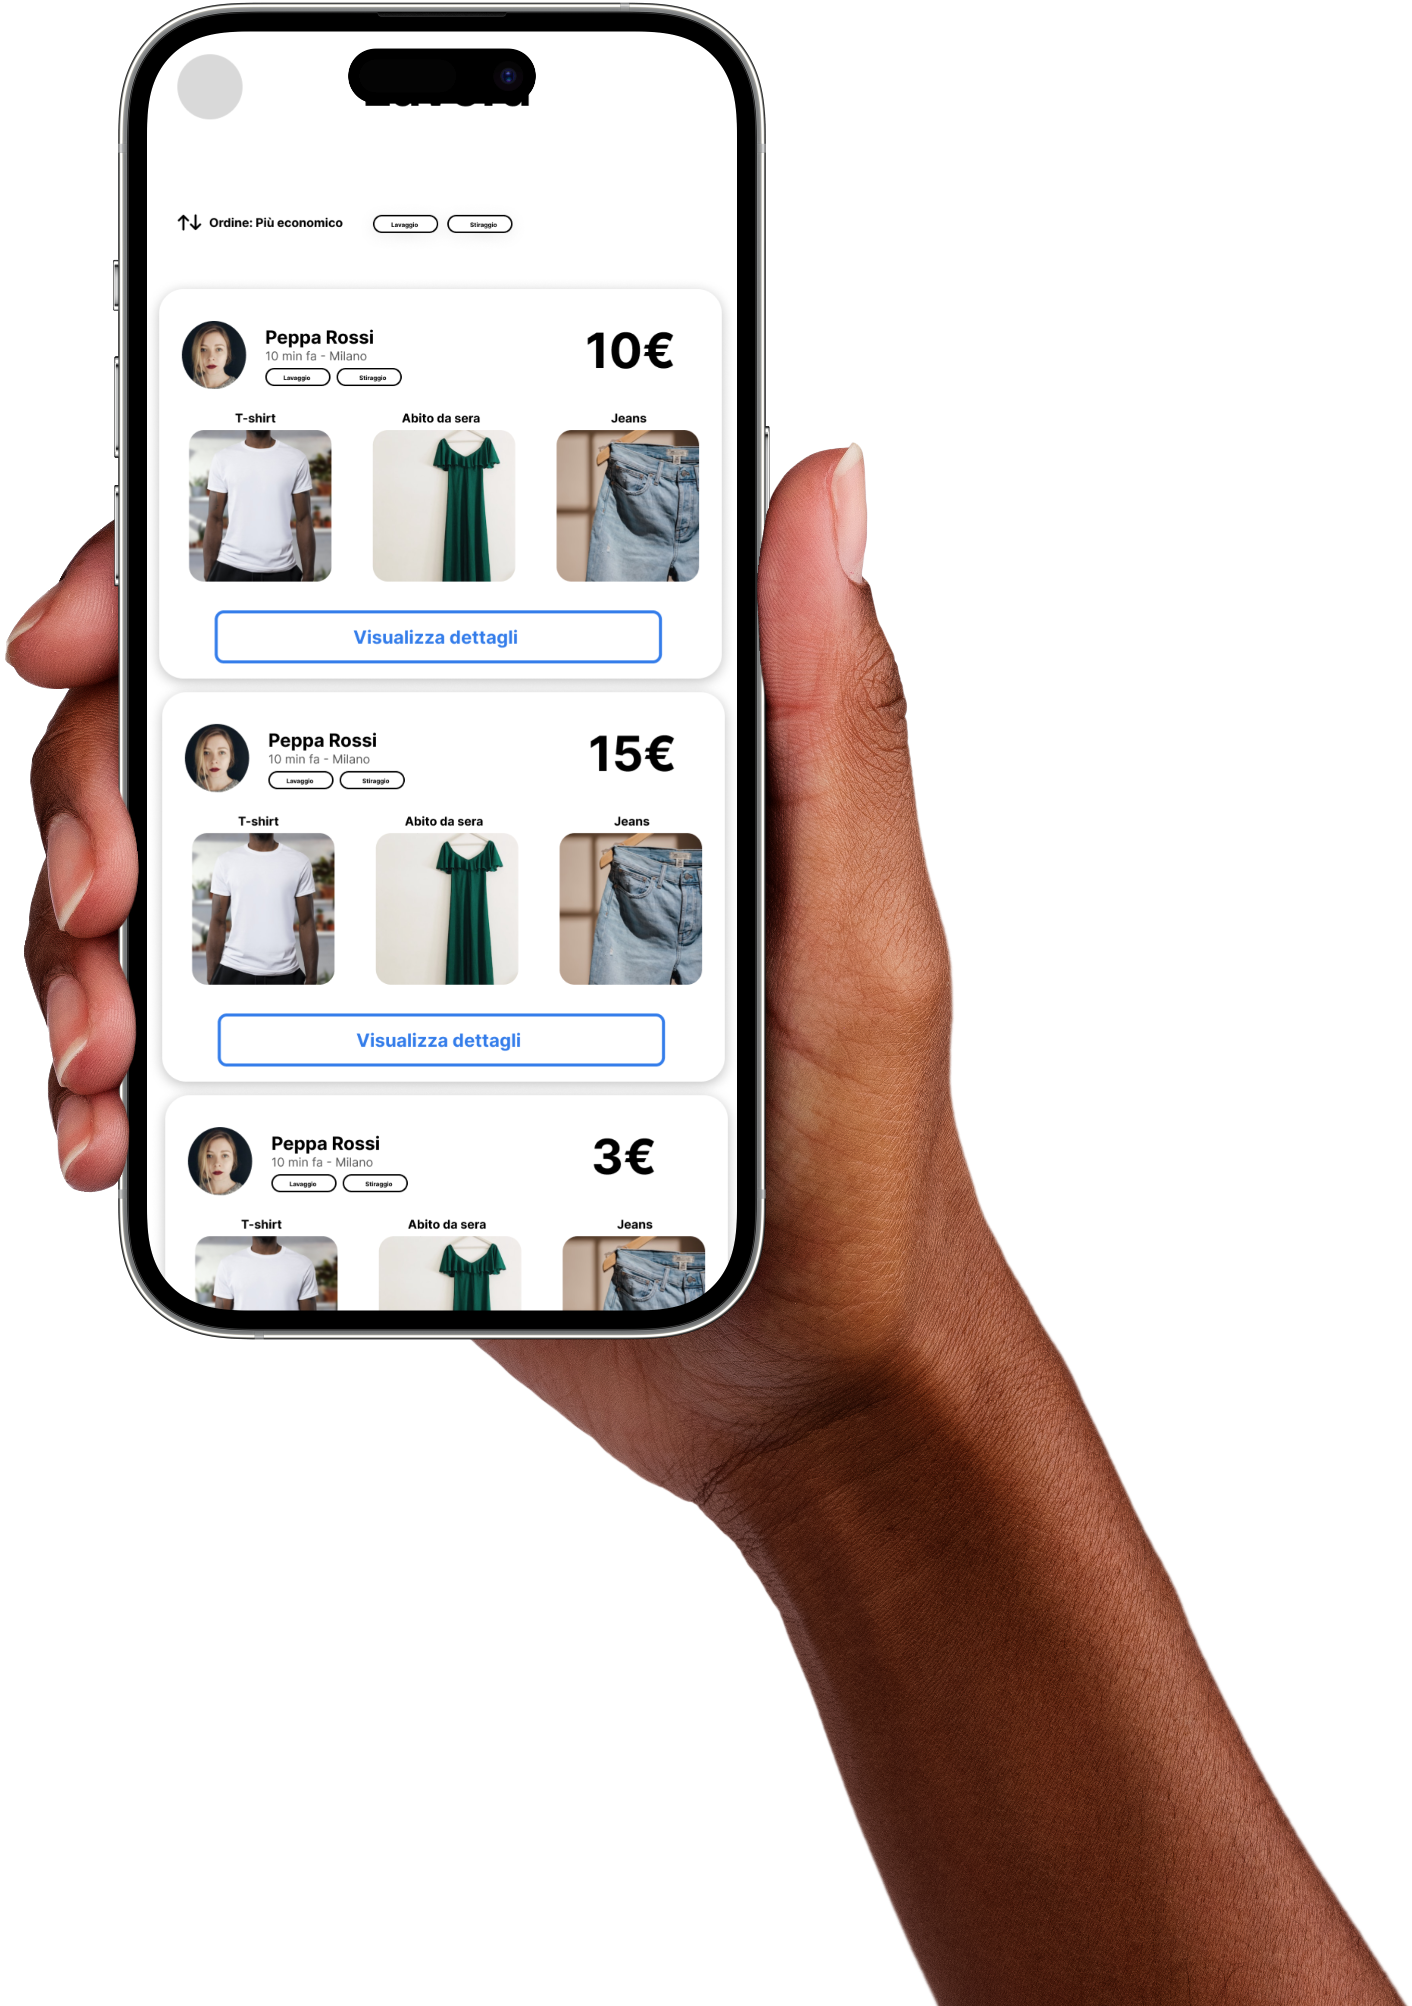
\includegraphics[scale=0.1]{../Images/mockup02.png}
\end{figure}
\begin{figure}[hbtp]
\caption{Detail Item Screen Mockup}
\centering
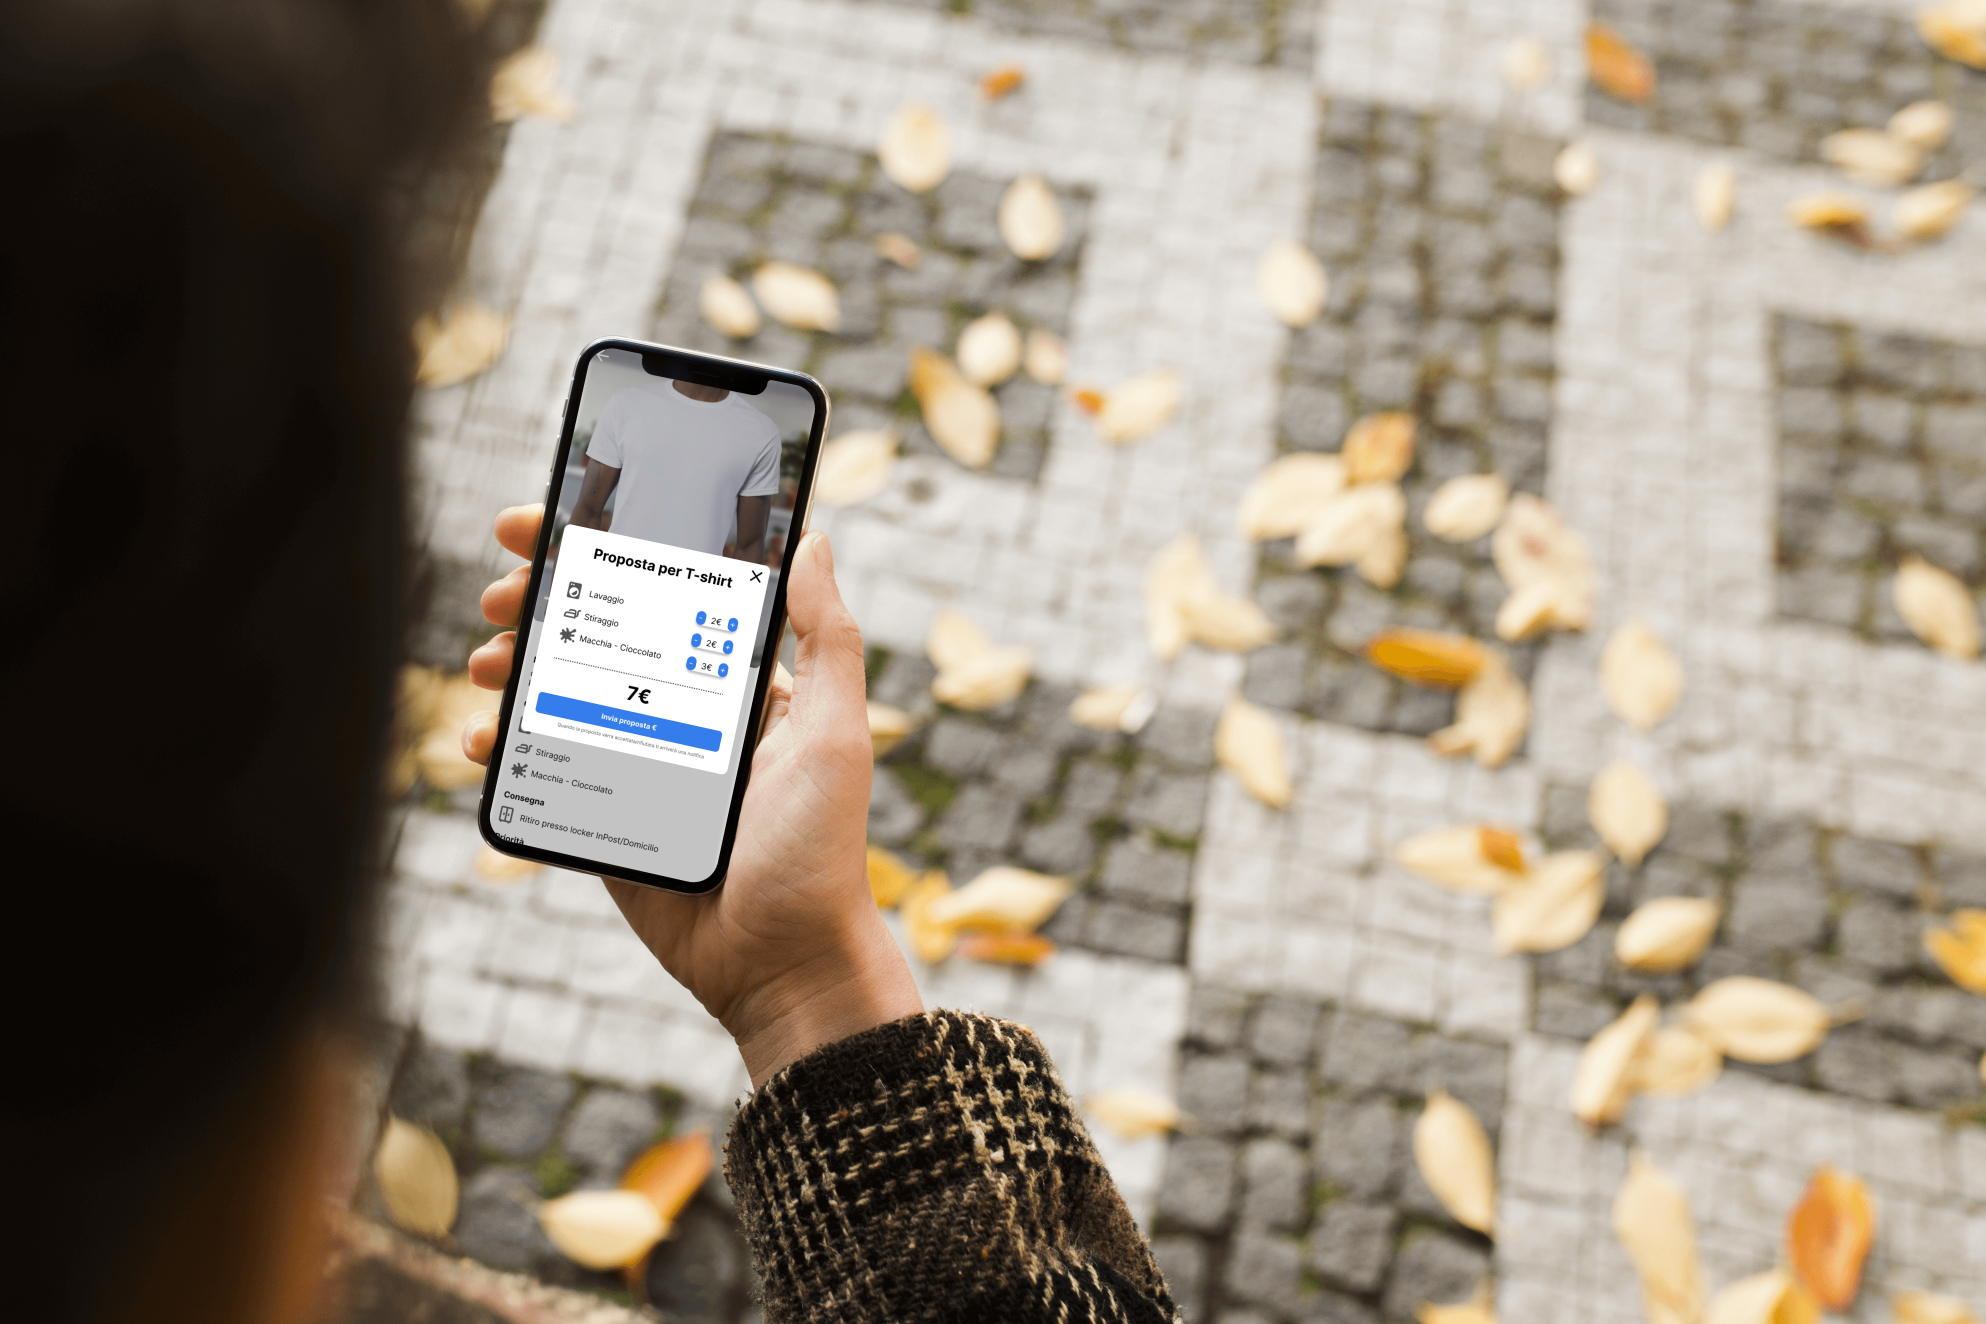
\includegraphics[scale=0.1]{../Images/mockup01.jpg}
\end{figure}
\section{A look into the market}
By doing a market analysis I obtained those main pillars:
\begin{itemize}
\item Buyers find this activity (washing/draining) time-consuming
\item Workers find this activity (washing/ironing) necessary and  have the skills to do it
\item Buyers prefer to find  someone who can take care their clothes
\item Workers make a profit for fulfilling these tasks
\end{itemize}
\section{Business Model}